\chapter{Case study: Ravenscar Avionics Platform}{``I ran out of
  altitude, airspeed and ideas all at the same time.''}{Chuck Yeager
    on why he ejected}
\label{chap:rap}
This appendix provides details of a large case study that was carried
out to test the AADL for its expressiveness, the capabilities of the
Ravenscar subset of Ada for programming of such systems, as well as
the code generation approach proposed.

Having been designed for safety-critical real-time systems, the \ada
runtime contains thread management, mutual exclusion and inter-thread
communication constructs. These are available directly as features in
the language, as opposed to---for example---the C language where such
features are furnished via an API that accesses these facilities
provided by the operating system.

In spite of these capabilities in the language and runtime,
practitioners in the 1980s were reluctant to use \ada 83 features for
tasking and synchronization~\cite{cornhill@irtaw87}. This stemmed from
the poor support for real-time constraints in generic \ada 83
runtimes, the inherent unpredictability of the rendezvous construct
(which was the only inter-task communication mechanism provided), as
well as a general reluctance on the part of practitioners to part with
established practice.

In order to demonstrate the feasibility of the \ada language and its
runtime for the construction of real-time systems, a case study was
carried out in the late 1980s. The Software Engineering Institute at
CMU, the Naval Weapons Center and IBM's Federal Sector Division
participated in the creation of the Generic Avionics Platform
(GAP). The work has been reported in~\cite{locke@rtss91}
and~\cite{locke@irtaw90}. The GAP is a software platform that
implements the Generic Avionics Software
Specification~\cite{locke@sei90}. It is sufficiently detailed to
faithfully model the Mission Control Computer (MCC) software of an
attack aircraft.

The GAP case study was implemented in \ada~83. \ada tasks were used to
implement different threads of control that implement the MCC
functions. Inter-task communication was carried out via rendezvous and
schedulability analysis was carried out using
RMA~\cite{liu@jacm73,liu@jacm73}. However, excessive use of the \ada
rendezvous renders the predictability and analyzability of the
application very hard.

The new tasking features introduced in \ada~95 such as protected
objects can replace the rendezvous to make real-time applications more
predictable. Also, the compliance with the Ravenscar concurrency
profile~\cite{burns@adalett04} of the new \ada~2005 standard can make
the application code statically analyzable. However, in an application
such as the GAP, where the number of threads is relatively large and
the communication topology complex (more than 15 threads with over 50
data-flows among them), writing code ``by hand'' that is compliant
with the Ravenscar Profile is a very tedious task. Therefore, a
generative approach must be adopted, where all the tasking and
inter-task communication code is automatically produced from a
well-defined model. Additionally, using a modeling language raises the
abstraction level of the application development process, making
source code management and traceability easier and more comprehensible
since there is a 1-to-1 correspondence between design artifact and
code artifact.

Consequently, the GAP case study was rearchitected using the
AADL. This allowed the automatic generation of a significant portion
of the code. The generated code contains the entire task-set defined
according to the architecture as well as the \ada protected object
constructs to handle the communication between tasks. This has
entailed foregoing the dangerous and unpredictable rendezvous. The
code produced is optimized for the application under development which
increases its performance and decreases its memory footprint. The
system developed is also compliant with the Ravenscar Profile, which
has rendered it analyzable for schedulability as well as safer, due to
the guaranteed absence of deadlock and bounded priority inversions.

The main purpose of this case study has been to demonstrate and
validate not only the \ada~2005 and the Ravenscar Profile towards the
construction of a relatively complex real-time system approximation,
but also the paradigm of code generation from \aadl and the associated
tooling developed. The advantages of this approach are manifold;
predictable real-time performance, safe construction of systems and
reduced time-to-market due to automatic generation of a significant
portion of code.

The rest of this appendix is structured as follows: In
Sec.~\ref{GAP} the GAP case study and its architecture is described
in detail. The redesign of the GAP is given in Sec.~\ref{design},
the benefits (and a few caveats) of the approach are presented in
Sec.~\ref{benefits}. Conclusions apprear in Sec.~\ref{conclusions}.

\section{The Generic Avionics Platform}
\label{GAP}
Before the redesign of the GAP architecture can be explained, an
introduction and overview of the classic platform is needed. The GAP
system models those aspects of a military aircraft that are essential
in successfully completing a mission. To be noted is the fact that a
digital flight control system---also called a fly-by-wire---is
\emph{not} a part of GAP. Furthermore, GAP models only the following
aspects:

\begin{itemize}
\item{Tasking configuration and its timing constraints;}
\item{Data-flow, including data types as well as their correct flow
  through subsystems and tasks;}
\item{Functional complexity, which is modeled by execution times of
  tasks.}
\end{itemize}

The avionics system consists of a set of sensors and subsystems
connected over a data bus---e.g., MIL-STD-1553B---to a central
computer, as in Fig.~\ref{fig:GAP}. The software for the mission
system computer performs a number of functions that aid in the
successful completion of the mission. The major sensors and other
hardware modeled in GAP include:

\begin{description}
\item[Air Data Computer:]{Provides barometric altitude data
  (air-pressure based altitude approximation), airspeed and magnetic
  heading data;}
\item[INS:]{The Inertial Navigation System provides best estimates of
  aircraft position using accelerometers and gyros, also provides body
  rates (roll, pitch and yaw);}
\item[Radar:]{This is the active radar which detects and tracks
  targets, both airborne and on the ground;}
\item[RALT:]{The Radar Altimeter provides accurate height measurements
  through electromagnetic pinging of the terrain underneath the
  aircraft;}
\item[RWR:]{The Radar Warning Receiver senses electromagnetic
  radiation over the aircraft's surface to detect radiating radars in
  the vicinity;}
\item[SMS:]{Combat aircraft carry weapons or pods (sensors, extra fuel
  etc.) on pylons under their wings and fuselage. These are all
  collectively labeled ``stores''. The Stores Management System keeps
  track of them, and releases them when the pilot so orders;}
\item[MPD:]{The Multi-Purpose Display is a CRT screen inside the
  cockpit that can be used to display various information according to
  the pilot's choice;}
\item[HOTAS:]{Hands On Throttle-And-Stick refers to the presence of
  various controls and switches on the throttle and joystick. This
  allows the pilot access to these buttons without his hands leaving
  the flight controls;}
\item[HUD:]{The Heads-Up-Display is a transparent display of vital
  information that does not obstruct the pilot's view;}
\item[Keyset:]{This includes all keys that may be pressed by the
  pilot that are not found on the HOTAS.}
\end{description}

\subsection{High-level Architecture}
The high-level GAP architecture, i.e.: the interconnection of the
various components and constituent artifacts, is given in
Fig.~\ref{fig:GAP}. All sensors (INS, ADC, Radar, RALT and RWR), as
well as the SMS are connected to the computer over a serial data bus
(MIL-STD-1553B). The HUD and MPD are connected over proprietary
display connectors. Keypresses from the HOTAS and Keyset are relayed
over a separate channel (another serial bus). In~\cite{locke@rtss91}
it is shown---as reproduced in Fig.~\ref{fig:GAP}---that there are two
distinct computers that make up the MCC; ``Display proc.'' and
``Mission Mgmt''. Since there is no mention of distribution elsewhere
in~\cite{locke@rtss91} it is assumed that they represent two distinct
subsystems on the same host.

\begin{figure}[htbp]
\centering
\includegraphics[scale=1.4]{figs/GAP_sys_arch}
\caption{The GAP system architecture: {\normalsize showing
  decomposition into sensors, subsystems and their interconnection,
  from~\cite{locke@rtss91}}}
\label{fig:GAP}
\end{figure}

The data-flow among these blocks is quite obvious. The set of sensors
(Radar, RALT, RWR, ADC and INS) sends data to the mission computer
over the serial bus. The format of said data is defined in detail in
the specification document~\cite{locke@sei90}. Also, in some instances
the mission computer sends commands to some of the sensors; such as
orders to the Radar to track a certain target. Orders, in the form of
release commands, are also sent to the SMS, which releases stores
according to those commands. SMS also sends status information to the
mission computer which apprises the pilot of the stores' situation.

\subsection{Software subsystems}
The software portions of the Mission Control Computer are described
here. From the point-of-view of Fig.~\ref{fig:GAP} this would be the
two boxes ``Display Proc.'' and ``Mission Mgmt''. The major software
subsystems and the tasks that comprise them which are modeled within
GAP, together with their tasking configurations, are given in
Table~\ref{tab:GAP_timing}. The timing constraints on these subsystems
are derived from human and hardware factors, these subsystems include:

\begin{description}
\item[Display:]{Updates the MPD as well as the HUD. Receives a myriad
  of data from the various other tasks including aircraft orientation,
  stores status, equipment status and aircraft position etc. All of
  which are displayed on either the HUD or the MPD (depending upon its
  mode);}
\item[Radar warning receiver:]{This subsystem receives threat data
  from the RWR, and may optionally send commands to it as a result of
  pilot input;}
\item[Radar control and tracking:]{Gathers target and track data from
  the radar. May optionally send commands to the radar to track
  specific targets as a result of pilot choice;}
\item[Navigation:]{Computes aircraft position and orientation. Sends
  steering commands if autopilot is activated;}
\item[Weapons subsystem:]{When activated, updates weapons
  ballistics. Also allows the designation of targets in conjunction
  with the radar subsystem. Furthermore, performs weapons release as a
  function of ballistics calculations, target designation and the
  pilot's keypress on the trigger;}
\item[Built-in-test:]{Performs diagnostics on the equipment.}
\end{description}

For detailed timing information refer to
Table~\ref{tab:GAP_timing}. The internal data-flow among software
subsystem tasks is rather complex and cannot be fully described here
for want of space. The interested reader may refer
to~\cite{locke@sei90}. An overview, however, is provided in
Fig.~\ref{fig:dataflow}.

There are also a number of deadline requirements stipulated on various
tasks (called ``jitter requirements'' in~\cite{locke@rtss91}). The
most important among these is the one on the task \texttt{Weapon
  release}. This requirement states that a release signal must be sent
to the SMS at most 5~ms after the ideal moment of release (either a
button depression by the pilot or calculated by the ballistics
task). This is ensured in GAP by giving the \texttt{Weapon release}
task the highest priority.

\begin{figure}
\centering
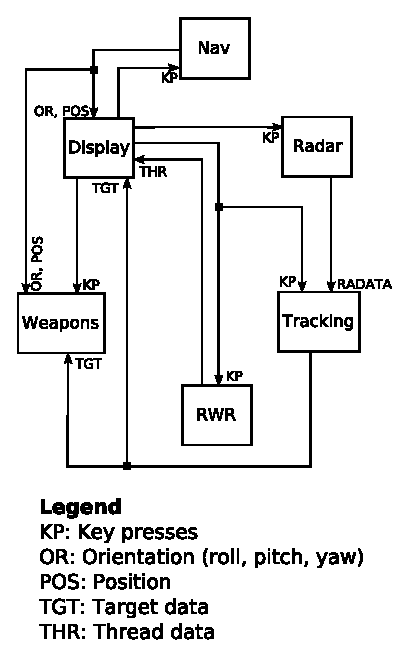
\includegraphics{figs/dataflow}
\caption{Data-flow in GAP: {\normalsize this figure shows the
    data-flow within the \emph{software} subsystems in the GAP mission
    control computer}}
\label{fig:dataflow}
\end{figure}

\begin{table}
\centering
\begin{tabular}{|l|l|l|l|l|}
\hline
\textbf{Subsystem} & \textbf{Task} & \textbf{Period/Response (ms.)} &
  \textbf{WCET} & \textbf{Utilization}\\
\hline
\multirow{5}{*}{Display} & Status Update & 200 & 3 & 1.50\\
 & Keyset & 200 & 1 & 0.50\\
 & Hook Update & 80 & 2 & 2.50\\
 & Graphic Display & 80 & 9 & 11.25\\
 & Stores Update & 200 & 1 & 0.50\\
\hline
RWR & Contact Mgmt. & 25 & 5 & 20.00\\
\hline
\multirow{2}{*}{Radar} & Target Update & 50 & 5 & 10.00\\
 & Target Filter & 25 & 2 & 8.00\\
\hline
\multirow{3}{*}{NAV} & Nav Update & 59 & 8 & 13.56\\
 & Steering Cmds & 200 & 3 & 1.50\\
 & Nav Status & 1000 & 1 & 0.10\\
\hline
Tracking & Target Update & 100 & 5 & 5.00\\
\hline
\multirow{3}{*}{Weapon} & Weapon Protocol & A 200 & 1 & 0.50\\
 & Weapon Release & A 200 & 3 & 1.50\\
 & Weapon Aim & A 50 & 3 & 6.00\\
\hline
BIT & Equ. Status Update & 1000 & 1 & 0.10\\
\hline
Data Bus & Poll Bus Devices & 40 & 1 & 2.50\\
\hline
\end{tabular}
\caption{GAP Timing Requirements: {\normalsize E is WCET (ms.) and U is
    utilization as a percentage}}
\label{tab:GAP_timing}
\end{table}

\section{Design}
\label{design}
The architecture modeling has been done totally in \aadl, code
generation has been carried out using the Ocarina\footnote{Available
  at \url{http://aadl.enst.fr/ocarina}} tool suite and is targeted to
the minimalist Ravenscar-compliant middleware
\polyorbhi{}~\cite{hugues@isorc07}. This middleware strictly follows
restrictions set by high-integrity applications on object orientation,
scheduling, memory use and task creation/destruction. It is developed
in \newada~\cite{arm05}. It is compliant with both the Ravenscar
profile and the High Integrity System Restrictions (Annexes~D and~H of
the \newada{} standard). Note that most restrictions are enforced at
compile time (no dispatching, no floating point, no allocator,
etc.). This simply yet efficiently enforces that no unwanted features
are used by the middleware, increasing the confidence in the code
generated while limiting its complexity. Code generated by \ocarina{}
also conforms to the same set of restrictions.

The GAP was redesigned using \aadl, which from now on shall be called
the Ravenscar Avionics Platform (or RAP). The design consists of the
software portion of the GAP modeled as a single ORK partition, with
the various functionalities implemented as threads within that
partition. Threads can be periodic or sporadic in Ravenscar, with
sporadic threads being those that are launched in response to an event
but with a stipulated minimum inter-arrival time for said events. Most
subsystem threads were directly translated to \aadl threads
(periodic).

However, there was one case identified where diverging from this
standard practice was necessary. This instance was the entire
``aperiodic'' weapon delivery subsystem. This subsystem remains
dormant until the pilot requests weapons delivery, at which point it
``wakes up'' and becomes a periodic system until weapon delivery is
finished. In~\cite{locke@sei90} it is made up of the threads
\texttt{Weapon trajectory} and \texttt{Weapon release}. These threads
were modeled in the Ravenscar context using an innovative
approach. The method employed was to reconfigure these threads as
sporadic with one important modification, they are able to send an
event to themselves in order to relaunch. They are activated or
awakened by an event from the pilot that signals weapons delivery,
which signifies the weapons delivery phase of the mission has been
started.

During this mission phase these threads send themselves an activation
event as the last action they take during their dispatch. In this
manner, they behave as periodic threads with a period equal to their
minimum inter-arrival time during this mission phase. When the phase
is over, they do not send the self-activation event at the end of
their dispatch and so must await an activation from elsewhere (another
instance of the event that signals a mode change \emph{into} the
weapons delivery phase). These threads were modeled in \aadl as shown
in Fig.~\ref{fig:mode_periodic}. The fact that the thread is sporadic
with a minimum inter-arrival time equal to the period of the GAP
thread ensures a periodic behavior during the weapons delivery phase
and does not cause a 100\% CPU utilization.

\begin{figure}
\centering

\includegraphics[scale=0.5]{figs/mode_periodic}
\caption{Mode-dependent periodic thread: {\normalsize all threads of
    the weapons subsystem are modeled according to this archetype,
    where the functional code of the thread requeues itself for
    periodic dispatch by sending an event to itself}}
\label{fig:mode_periodic}
\end{figure}

The event connection from output event port \texttt{Do\_Relaunch} to
the input event port \texttt{Relaunch} is converted to an event type
received by the protected object on which this thread waits and an API
procedure to send this event, respectively. The input event port
\texttt{Mode\_Activation} is the port over which an incoming event
will signal that this periodic task now needs to be activated.

The system also models the data coming in from various sensors in
order to carry out hardware-in-the-loop (HIL) simulation:

\begin{itemize}
\item The ADC (Air Data Computer);
\item The RALT (Radar Altimeter);
\item The INS (Inertial Navigation System);
\item The Radar and the RWR (Radar Warning Receiver).
\end{itemize}

Also modeled are the key presses of the pilot coming from both the MPD
(Multi-Purpose Display) and the HOTAS (Hands On Throttle And Stick)
subsystems. All HIL threads have been separated out into a different
partition which simplifies the schedulability analysis of the RAP
system threads.

The entire \aadl system model is available at
\hbox{\url{http://aadl.enst.fr/RAP}} for download. Also available is a
graphical representation of the model.

\section{Benefits}
\label{benefits}
As stated, the purpose of any modeling activity in the domain of
computing can be reduced to one or more of three categories:
documentation, analysis and code generation. The approach
taken---either incidentally or intentionally---achieves all three
above-mentioned goals of modeling. Documentation occurs incidentally
as a consequence of using AADL. Any architecture description language
used will serve to document the system architecture. Analysis is
intentional, since the Cheddar scheduling analysis
tool~\cite{singhoff@alj04} has been used to carry this out. Cheddar
allows the schedulability analysis of AADL system models. Code
generation is also intentional as it is the primary axis of the
research.

\subsection{Analyses}
As previously stated, the use of a model driven approach to building
high-integrity systems allows the application of several analyses on
the model before code generation. The major analysis carried out on
the RAP system model is of course that of real-time schedulability using
Cheddar. Two different analyses were carried out, the Rate Monotonic
Analysis as well as the Response Time Analysis.

\subsubsection{Rate Monotonic Analysis (RMA)}
Based on the WCET execution times that have been provided
by~\cite{locke@rtss91}, the processor utilization factor with thread
periods is $0.86$ which means $86\%$ of CPU usage. It is slightly
different from the $84\%$ of CPU usage factor found
in~\cite{locke@rtss91} because in the RAP analysis the \texttt{Weapon
  trajectory} and \texttt{Weapon release} tasks were taken into
account which are not always active. This factor is greater than
$0.709$, thus it cannot be proven that the task set is schedulable
using RMA. However, the Cheddar real-time simulator can deduce that
our task set is schedulable. This is due to the well-known
critical-zone theorem given in~\cite{liu@jacm73, sha@ieeeproc94}. This
theorem states that if a task meets its first deadline when it and all
higher priority tasks were launched at the same time, then it will
meet all its subsequent deadlines.

\subsubsection{Response Time Analysis (RTA)}
The processor utilization factor with thread deadlines is $0.86$ which
means $86\%$ of CPU usage (in the RAP model, deadlines are equal to
periods). This factor is greater than $0.709$, thus it cannot be
proven that the task set is schedulable. Using the Cheddar real-time
simulator, and based on a worst-case task response time it can be
deduced that all task deadlines will be met. Below is a part of the
output of the Cheddar analyzer applied on the RAP model: {\small
\begin{verbatim}
Scheduling feasibility, Processor rap.leon.s_cpu :

1) Feasibility test based on the processor 
   utilization factor :

- The base period is 118000 (see [18], page 5).
- 15447 units of time are unused in the base 
  period.
- Processor utilization factor with deadline is 
  0.86909 (see [1], page 6).
- Processor utilization factor with period is 
  0.86909 (see [1], page 6).
- In the preemptive case, with RM, we can not 
  prove that the task set is schedulable because 
  the processor utilization factor 0.86909 is more 
  than 0.70941 (see [1], page 16, theorem 8).

2) Feasibility  test based on worst case task 
   response time :

- Bound on task response time :  (see [2], page 3, 
  equation 4).
    rap.leon.software.builtin_test => 142
    rap.leon.software.steering => 141
    rap.leon.software.weapon_selection => 138
    rap.leon.software.weapon_release => 100
    rap.leon.software.mpd_status_display => 75
    rap.leon.software.mpd_stores_display => 72
    rap.leon.software.keyset => 50
    rap.leon.software.target_tracking => 49
    rap.leon.software.hud_display => 44
    rap.leon.software.mpd_tactical => 42
    rap.leon.software.ac_flight_data => 22
    rap.leon.software.weapon_trajectory => 14
    rap.leon.software.hotas => 11
    rap.leon.software.radar_control => 10
    rap.leon.software.rwr_threat_response => 5
- All task deadlines will be met : the task set is 
  schedulable.
\end{verbatim}
}
\subsection{Code generation}
Framework code was automatically generated for a working system from
the RAP system model in AADL. This framework for the application was
then ``fleshed out'' with functional code that was hand-written to
model the computational complexity of each thread as well as the data
flows within the system. Table~\ref{SLOCs} summarizes the code size
for the RAP application (15 communicating threads). The size of the
\aadl textual model is also given for comparison.

\begin{table}
\centering
\begin{tabular}{|l|r|}
\hline
\textbf{Component} & \textbf{Source Lines of Code (SLOCs)}\\
\hline
AADL model         & $765$\\
User code          & $378$\\
Middleware         & $1255$\\
Generated code     & $7243$\\
\hline
\end{tabular}
\caption{Source code size}
\label{SLOCs}
\end{table}

Given the development process employed, most code is automatically
generated for an \aadl{} model ($81\%$ in the case of RAP). The code
in the middleware handles simple types: messages, protocol,
transport. Generated code adds tasking constructs required to execute
the application: transport handlers, application activities,
marshallers, naming tables, etc. This enables the optimization of the
performance and the footprint of the application since the greatest
part of the code is customized for the current application. The memory
footprint of the executable corresponding to the RAP application is
1.2 Mb using both a native \ada compiler and the GNAT for LEON Ada
compiler. Given the large number of threads and interfaces in the
application, the executable size is acceptable for an embedded system.

The ratio of user vs. generated code will be higher for a deployed
application. This is so because in RAP the functional complexity was
modeled only using busy waiting within tasks (similar to the original
GAP case study). This rendered the functional code quite
simple. However, in a real mission control computer system, the user
code will be larger as it will contain the actual
functionality. However, it bears stating that the user code in this
case will be \emph{purely} sequential and will thus not have any
consequence upon---or error related to--- concurrency. Also, code
generation formalisms for sequential code exist as well, which allow
the generation of verified functional code. One of these, SCADE, can
be used to generate C and \ada code compatible with that generated by
the Ocarina toolset\footnote{Complementary work on this topic has been
  accepted for publication in the ERTS'08 conference}.

From the high-integrity systems point-of-view, the use of automatic
code generation in the development process is doubly
beneficial. Firstly, it drastically reduces the prototyping time of
DRE systems~\cite{hugues@rsp07}. Secondly, the fact that the generated
code is a combination of a relatively small set of extensively tested
design patterns, the analysis and review (e.g., in the context of the
DO-178B standard~\cite{do178b}) of this code is easier than that of
hand-written code.

Unfortunately, it was not possible to obtain the code for the original
GAP project due to it having been lost. However,
from~\cite{locke@rtss91, locke@sei90} it can be noted that the
original GAP system carried out on average 277 rendezvous/sec, which
has been reduced to 0 in the RAP through the use of protected
objects. The use of the priority ceiling protocol on each protected
object entails that there is no deadlock/livelock and that priority
inversion is bounded \emph{and} calculable for each protected object
being accessed by a task.

\subsection{Design Documentation}
The use of an architecture description language such as the \aadl
results in a very easily communicable system design. Quite a bit of
difficulty was encountered in deciphering the specification document
of the GAP~\cite{locke@sei90}. On the other hand, the same system
design given in \aadl is very intuitive and easy to
understand. Whereas in the GAP specification document all thread
input/output and timing characteristics were explained in text, the
RAP now provides a model where they are formally enunciated:

\begin{itemize}
\item
  The interface of each thread is precisely defined in the
  \emph{features} section, which states what data it receives,
  transmits and what is the type of said data interchange;

\item
  The timing characteristics of each thread are given as \aadl
  properties of that thread:
  \begin{itemize}
  \item
    The dispatching protocol for the thread, whether it is periodic or
    sporadic;

  \item
    The thread's worst-case execution time;

  \item
    Its period (for a periodic thread) or its minimum inter-arrival
    time (for a sporadic thread);

  \item
    The deadline for the thread.
  \end{itemize}
  
\item
  The connections between the ports on various threads gives a very
  clear picture of the communication topology and by extension, the
  data-flow through the entire system. This was a major problem in
  understanding the original GAP specification.
\end{itemize}

\subsection{Criticisms}
There exist, however, a few restrictions that result from the use of
this paradigm. Some of these restrictions stem from compliance with
the Ravenscar Profile, some from the use of AADL as a design vehicle,
and some from the Ada language itself. The first is that task
priorities cannot be changed dynamically. This is due to the Ravenscar
Profile, the reason being that changing priorities breaks the
schedulability analysis performed \emph{\`a priori}. However, this can
be overcome by using an approach presented in~\cite{puente@adalett01},
which involves decoupling the \emph{job} from the \emph{task}. The
code invoked by a task is reattached to another task the priority of
which is correct for the new period.

The Ravenscar profile---as well as AADL---do not allow the
creation/destruction of tasks. This means that in case tasks are made
inactive, using an approach as described in Sec.~\ref{design} for the
weapons tasks, they will still remain in memory.

A final restriction is that synchronous communication between tasks
(RPCs) cannot be used. This is due also to the Ravenscar Profile,
enforced to ease schedulability analysis and render the application
more secure (in case a server thread crashes). This can be overcome by
avoiding the RPC paradigm itself in the design and using asynchronous
constructs in its place.

However, all of these restrictions can be seen as an enforcement of
``best practices'' within the embedded and real-time domain as they
lead to systems that are easier to analyze, simpler to construct and
safer to execute.

\section{Conclusions}
\label{conclusions}
An existing case study of an avionics system was rearchitected using
the AADL and code was generated for it automatically. The main reason
for undertaking this case study was to validate and demonstrate the
usability of the whole gamut of technology towards the construction of
real-time systems in general and aerospace/avionics systems in
particular. The aforementioned technology being of course the Ada
95/2005 language, the Ravenscar Profile and---most importantly---the
automatic code generation paradigm and tooling. To the knowledge of
the author, this case study is the largest effort carried out to date
for the generation of code from AADL. It is a substantial analysis
effort as well. However, it is not the \emph{largest} AADL model
analysis effort. The largest AADL model analyzed has been a
re-engineered fly-by-wire model for a helicopter flight control system
carried out by Honeywell; at reportedly 22,000 lines of AADL, it
dwarfs this case study's approximately 1000 lines of AADL by an order
of magnitude.

%%% Local Variables:
%%% mode: latex
%%% mode: flyspell
%%% TeX-master: t
%%% End:
